% Gemini theme
% See: https://rev.cs.uchicago.edu/k4rtik/gemini-uccs
% A fork of https://github.com/anishathalye/gemini

\documentclass[final]{beamer}

% ====================
% Packages
% ====================

\usepackage[T1]{fontenc}
\usepackage{lmodern}
\usepackage[size=custom,width=121.92,height=60.96,scale=1.0]{beamerposter}
\usetheme{gemini}
% \usecolortheme{uchicago}
\usecolortheme{stanford}
\usepackage{graphicx}
\usepackage{booktabs}
\usepackage{tikz}
\usepackage{pgfplots}
\pgfplotsset{compat=1.17}

% ====================
% Lengths
% ====================

% If you have N columns, choose \sepwidth and \colwidth such that
% (N+1)*\sepwidth + N*\colwidth = \paperwidth
\newlength{\sepwidth}
\newlength{\colwidth}
\newlength{\widecolwidth}
\setlength{\sepwidth}{0.0001\paperwidth}
\setlength{\colwidth}{45cm}
\setlength{\widecolwidth}{65cm}

\newcommand{\separatorcolumn}{\begin{column}{\sepwidth}\end{column}}


\title{From Possible to Pause-able: Children's hesitancy may mark implicit skepticism of incorrect intuitive beliefs}


\author{Adani B. Abutto \inst{1, 2} \and Igor Bascandziev \inst{1} \and Caren Walker \inst{3} \and Elizabeth Bonawitz \inst{1}}

\institute[shortinst]{\inst{1} Harvard Graduate School of Education \samelineand \inst{2} Stanford University  \samelineand \inst{3} UC San Diego}

% ====================
% Footer (optional)
% ====================

\footercontent{
  \href{https://adaniabutto.com}{stanford.edu/\~ aabutto} \hfill
	Biennial Meeting of the Cognitive Development Society \hfill
  \href{mailto:aabutto@stanford.edu}{aabutto@stanford.edu}}

% ====================
% Logo (optional)
% ====================

% use this to include logos on the left and/or right side of the header:
 \logoright{
\includegraphics[height=8cm]{stanford_logos/hgse_logo_clear.png}}
 \logoleft{
\includegraphics[height=8cm]{stanford_logos/CoCoDev_Logo.png}}

% ====================
% Body
% ====================

\begin{document}

\begin{frame}[t]
\begin{columns}[t]
\separatorcolumn

\begin{column}{\colwidth}

  \begin{block}{BACKGROUND}

    \begin{itemize}
      \item Young children assert that invisible but material things, such as air, are immaterial
      \item While learners' \textbf{naive beliefs are revised} throughout development, \textbf{some aspects} are \textbf{retained} in adulthood
      \item Even \textbf{expert adults regress to} responding in line with their \textbf{naive beliefs} when put under time pressure 
    \end{itemize}
    
\begin{alertblock}{Research Question}

    Curabitur eu libero vehicula, cursus est fringilla, luctus est. Morbi
    consectetur mauris quam, at finibus elit auctor ac.

  \end{alertblock}

  \end{block}

  \begin{block}{PROCEDURE}

    Nam vulputate nunc felis, non condimentum lacus porta ultrices. Nullam sed
    sagittis metus. Etiam consectetur gravida urna quis suscipit.

    \begin{figure}
      \centering
	{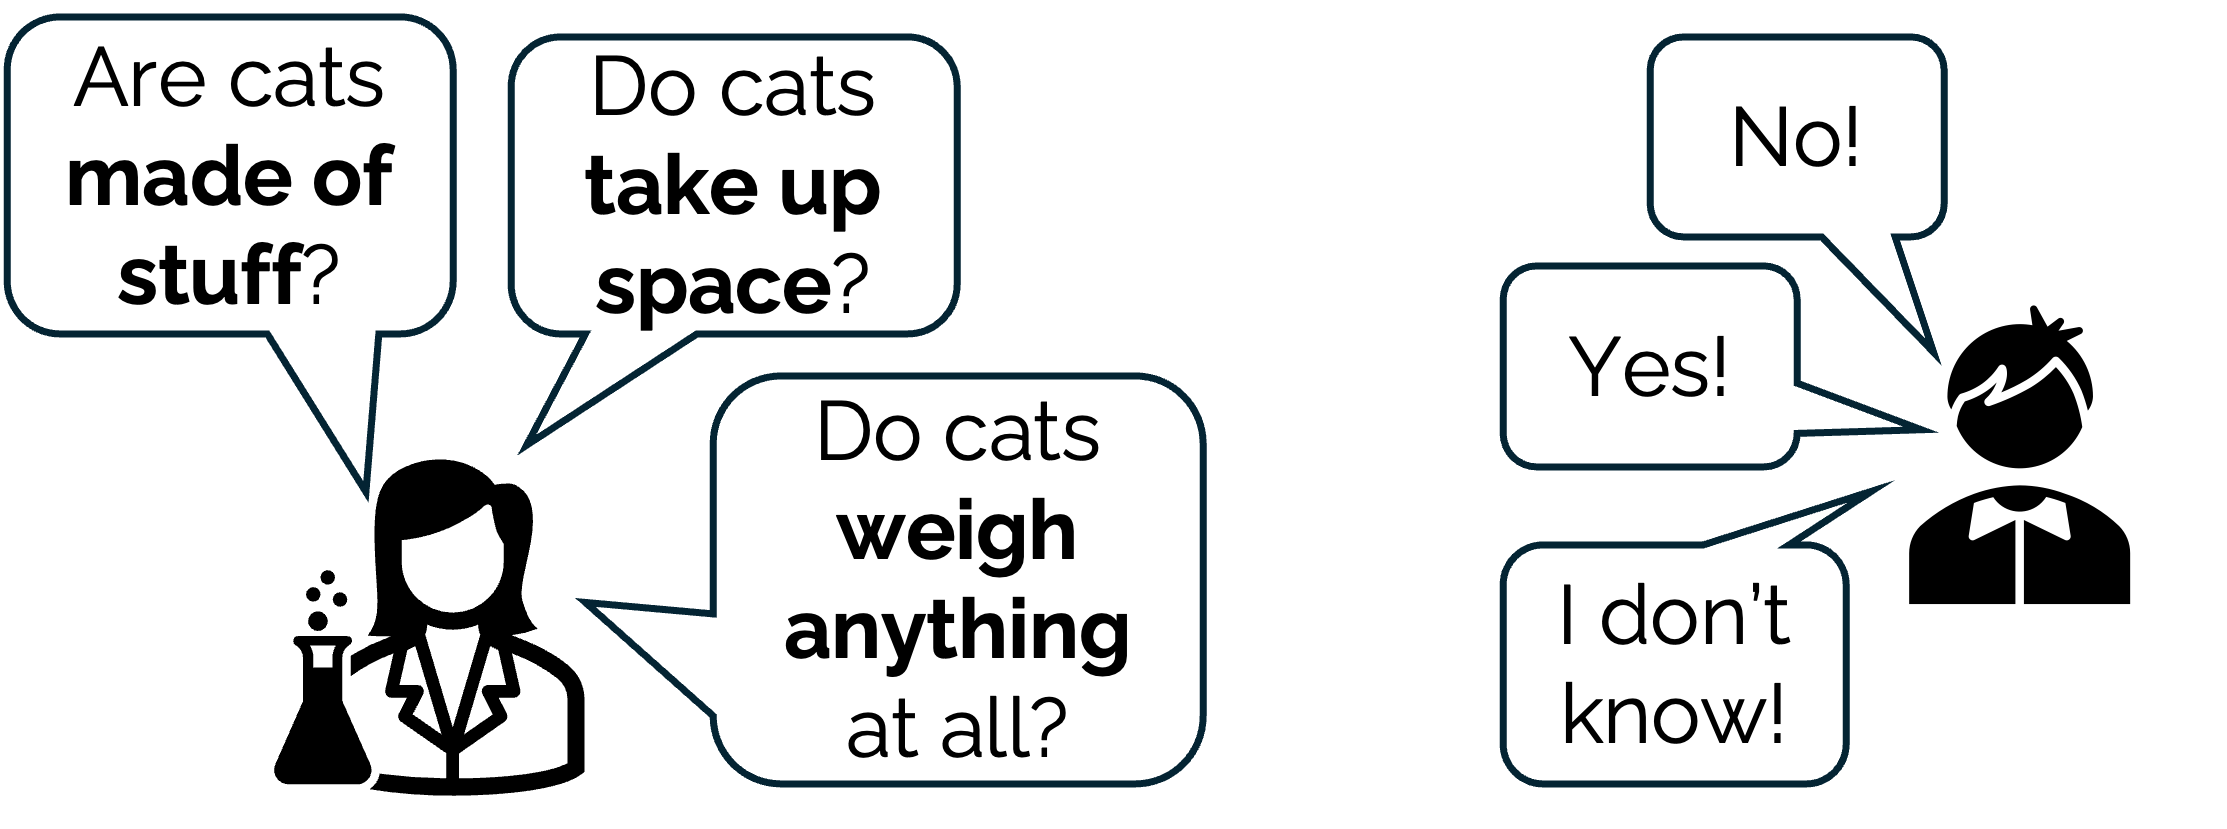
\includegraphics[height=12cm]{images/procedure1.png}}
      \caption{A figure caption.}
    \end{figure}

    Eget augue porta, bibendum venenatis tortor.

  \end{block}

\end{column}

\separatorcolumn

\begin{column}{\widecolwidth}

  \begin{block}{RESULTS}
  
  \emph{N} = 79 five- to nine-year-olds

    \begin{figure}
      \centering
      \begin{tikzpicture}
        \begin{axis}[
            scale only axis,
            no markers,
            domain=0:2*pi,
            samples=100,
            axis lines=center,
            axis line style={-},
            ticks=none]
          \addplot[red] {sin(deg(x))};
          \addplot[blue] {cos(deg(x))};
        \end{axis}
      \end{tikzpicture}
      \caption{Another figure caption.}
    \end{figure}

  \end{block}
    
      \begin{block}{DISCUSSION \& FUTURE DIRECTIONS}

    Nam vulputate nunc felis, non condimentum lacus porta ultrices. Nullam sed
    sagittis metus. Etiam consectetur gravida urna quis suscipit.

    \begin{itemize}
      \item \textbf{Mauris tempor} risus nulla, sed ornare
      \item \textbf{Libero tincidunt} a duis congue vitae
      \item \textbf{Dui ac pretium} morbi justo neque, ullamcorper
    \end{itemize}

    Eget augue porta, bibendum venenatis tortor.

  \end{block}

  \begin{block}{REFERENCES}

    \nocite{*}
    \footnotesize{\bibliographystyle{plain}\bibliography{poster}}

  \end{block}

\end{column}
\end{columns}
\end{frame}

\end{document}
